\documentclass[class={IEEEtran}]{standalone}

\usepackage{amsmath}
\usepackage{tikz}
\usepackage{pifont}

\newcommand{\whiteding}[1]{\large{\ding{\numexpr171+#1\relax}}}

\pagestyle{empty}

\usetikzlibrary{shapes.geometric,shapes.arrows,positioning,calc,arrows.meta,math}

\tikzset{AGENT/.style={rectangle,minimum width=6.5em,minimum height=3.5ex,draw,semithick,align=flush center, anchor=north}}
\tikzset{ACTION/.style={rectangle,rounded corners,draw,semithick,align=flush center,fill=white}, anchor=north}
\tikzset{ARROW/.style={thick, -stealth}}
\tikzset{DARROW/.style={<->,>=latex, line width=4ex, gray!20}}
\tikzset{PREPARATION/.style={rectangle,draw,semithick,align=flush center,fill=white,dashed, anchor=north}}


\begin{document}
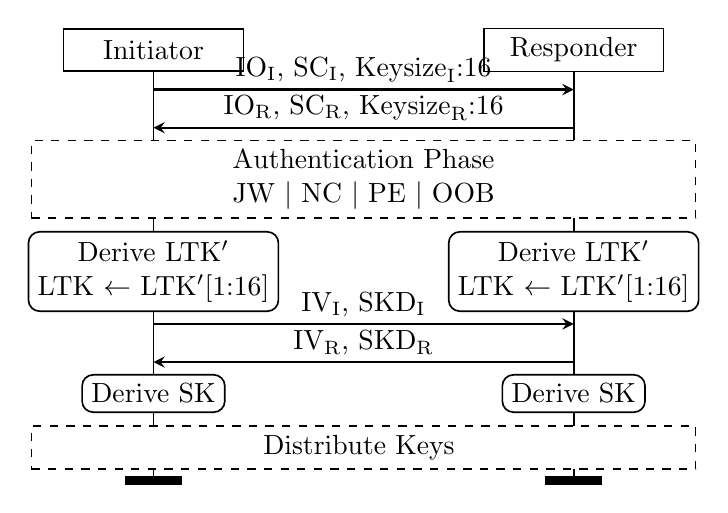
\begin{tikzpicture}

\node[AGENT] (n_initiator) {Initiator};
\node[AGENT, right=0.25\textwidth of n_initiator] (n_responder) {Responder};

\coordinate (end_initiator) at ($(n_initiator.south)+(0,-34ex)$);
\draw[semithick] (n_initiator.south) -- (end_initiator);
\draw[fill=black] ($(end_initiator)+(-1em,0)$) rectangle ($(end_initiator)+(1em,-0.6ex)$);

\coordinate (end_responder) at ($(end_initiator-|n_responder)$);
\draw[semithick] (n_responder.south) -- (end_responder);
\draw[fill=black] ($(end_responder)+(-1em,0)$) rectangle ($(end_responder)+(1em,-0.6ex)$);

\coordinate (c_middle) at ($(n_initiator.south)!0.5!(n_responder.south)$);
% \node[PREPARATION, minimum width=24em] (n_prep) at ($(c_middle)+(0, -1ex)$) {Establish Link Layer Connection};

\coordinate (c_init_pair_req) at ($(n_initiator.south-|n_initiator)+(0,-1.5ex)$);
\coordinate (c_res_pair_req) at ($(c_init_pair_req-|n_responder)$);
\draw[ARROW] (c_init_pair_req) -- (c_res_pair_req) node[midway,above=-0.3ex]{$\text{IO}_\text{I}$, $\text{SC}_\text{I}$, $\text{Keysize}_\text{I}$:16};

\coordinate (c_res_pair_rsp) at ($(c_res_pair_req)+(0,-3.2ex)$);
\coordinate (c_init_pair_rsp) at ($(c_res_pair_rsp-|n_initiator)$);
\draw[ARROW] (c_res_pair_rsp) -- (c_init_pair_rsp) node[midway,above=-0.3ex]{$\text{IO}_\text{R}$, $\text{SC}_\text{R}$, $\text{Keysize}_\text{R}$:16};
\node[PREPARATION, minimum width=24em] (n_user) at ($(c_res_pair_rsp-|c_middle)+(0,-1ex)$) {
    Authentication Phase \\
    JW $|$ NC $|$ PE $|$ OOB
};

\node[ACTION] (n_initiator_ltk) at ($(n_user.south-|n_initiator)+(0,-1ex)$) {Derive LTK$'$ \\ LTK $\leftarrow$ LTK$'$[1:16]};
\node[ACTION] (n_responder_ltk) at ($(n_user.south-|n_responder)+(0,-1ex)$) {Derive LTK$'$ \\ LTK $\leftarrow$ LTK$'$[1:16]};

\coordinate (c_init_ltk) at ($(n_initiator_ltk.south)+(0,-1ex)$);
\coordinate (c_res_ltk) at ($(c_init_ltk-|n_responder)$);
\draw[ARROW] (c_init_ltk) -- (c_res_ltk) node[midway,above=-0.3ex]{$\text{IV}_\text{I}$, $\text{SKD}_\text{I}$};

\coordinate (c_res_ltk) at ($(c_res_ltk)+(0,-3.2ex)$);
\coordinate (c_init_ltk) at ($(c_res_ltk-|n_initiator)$);
\draw[ARROW] (c_res_ltk) -- (c_init_ltk) node[midway,above=-0.3ex]{$\text{IV}_\text{R}$, $\text{SKD}_\text{R}$};

\node[ACTION] (n_initiator_sk) at ($(c_init_ltk)+(0,-1ex)$) {Derive SK};
\node[ACTION] (n_responder_sk) at ($(c_res_ltk)+(0,-1ex)$) {Derive SK};

\node[PREPARATION, minimum width=24em] (n_distribution) at ($(n_responder_sk.south-|c_middle)+(0,-1ex)$) {
    Distribute Keys
};

\end{tikzpicture}

\end{document}
